% Copyright (c) 2026 Islam Ibrahim. All rights reserved.

\documentclass[tikz,border=8pt]{standalone}
\usepackage[T1]{fontenc}\usepackage{lmodern}\usepackage{amsmath}\usepackage{tikz}
\usetikzlibrary{arrows.meta,positioning,calc}
\begin{document}
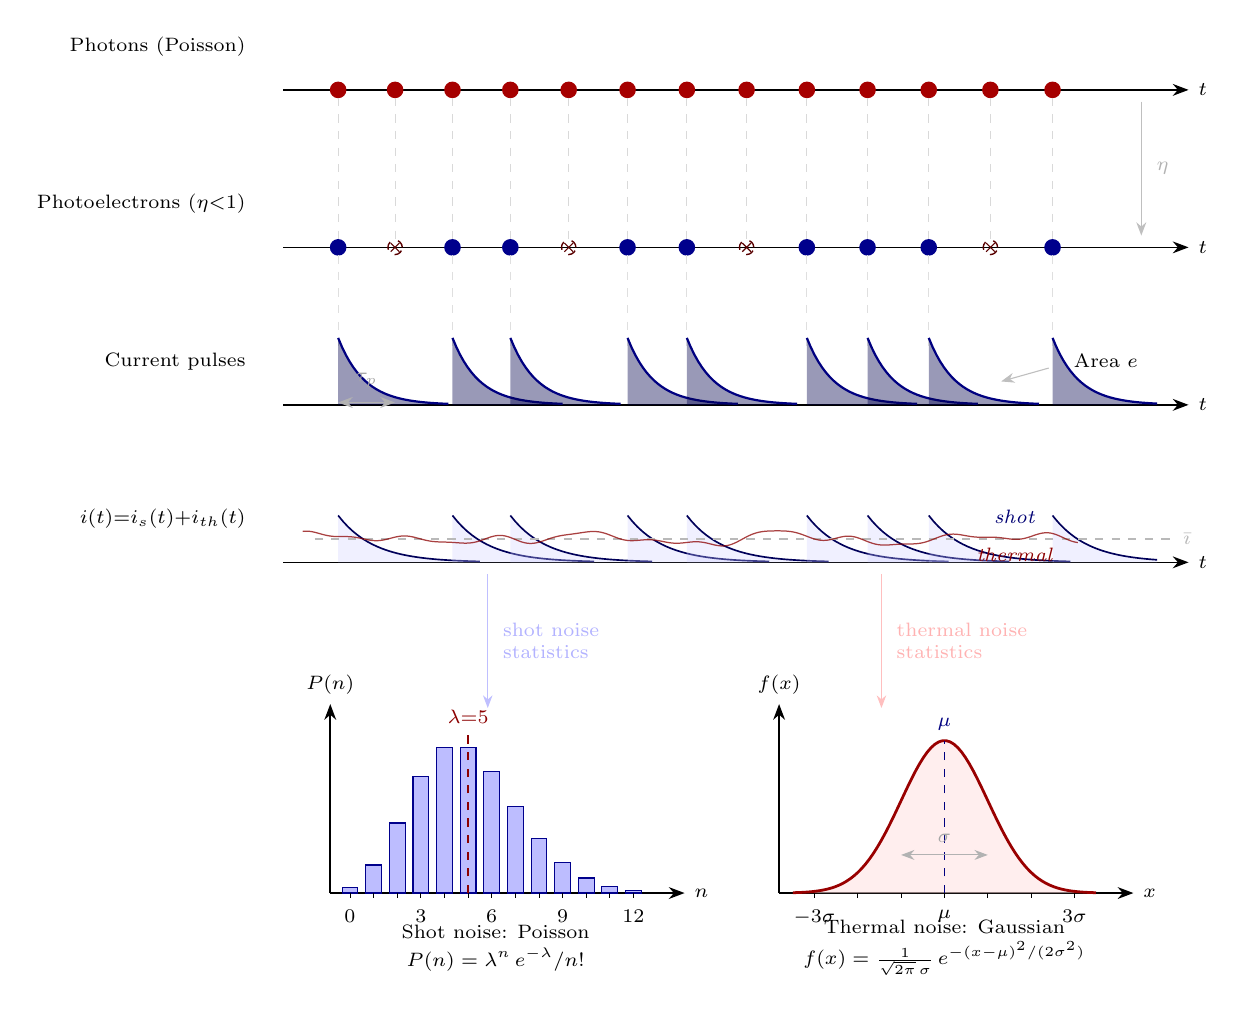
\begin{tikzpicture}[font=\small\rmfamily,>=Stealth,
  lbl/.style={font=\scriptsize\rmfamily},
  ax/.style={line width=0.6pt,->},
  seg/.style={line width=0.8pt},
]

\def\TW{11.0}
\def\rowgap{2.0}
\def\pulseH{0.85}
\def\Narr{13}

% Random survival mask: 1 = detected, 0 = lost (Bernoulli thinning)
% Quantum efficiency eta ~ 0.69 (9 of 13 survive)
\def\survive{{1,0,1,1,0,1,1,0,1,1,1,0,1}}

%% ================================================================
%% ROW 3 — Photons (Poisson arrivals)
%% ================================================================
\pgfmathsetmacro{\ybiii}{\rowgap*3}
\draw[ax] (-0.1,\ybiii)--(\TW+0.4,\ybiii) node[right,lbl]{$t$};
\node[lbl,align=right,left=10pt] at (-0.1,\ybiii+0.55) {Photons (Poisson)};

\foreach \k in {0,...,12}{%
  \pgfmathsetmacro\xp{0.6+\k*0.72+(\k*\k*0.003)}%
  \fill[red!65!black] (\xp,\ybiii) circle (3.0pt);
}

%% ================================================================
%% ROW 2 — Photoelectrons with random loss (Bernoulli thinning)
%%   Each photon is independently lost with probability 1 - eta.
%%   The surviving count is still Poisson (thinned process).
%% ================================================================
\pgfmathsetmacro{\ybii}{\rowgap*2}
\draw[ax] (-0.1,\ybii)--(\TW+0.4,\ybii) node[right,lbl]{$t$};
\node[lbl,align=right,left=10pt] at (-0.1,\ybii+0.55)
  {Photoelectrons ($\eta{<}1$)};

\foreach \k in {0,...,12}{%
  \pgfmathsetmacro\xp{0.6+\k*0.72+(\k*\k*0.003)}%
  \pgfmathsetmacro\sv{\survive[\k]}%
  % Dashed guide line from photon row
  \draw[line width=0.3pt,gray!30,dashed]
    (\xp,\ybiii-0.10)--(\xp,\ybii+0.10);
  \ifdim\sv pt>0.5pt
    % Surviving: solid blue dot
    \fill[blue!55!black] (\xp,\ybii) circle (3.0pt);
  \else
    % Lost: dashed hollow circle with cross
    \draw[red!35!black,dashed,line width=0.5pt]
      (\xp,\ybii) circle (2.6pt);
    \draw[red!35!black,line width=0.4pt]
      (\xp-0.055,\ybii-0.055)--(\xp+0.055,\ybii+0.055)
      (\xp-0.055,\ybii+0.055)--(\xp+0.055,\ybii-0.055);
  \fi
}

% Eta annotation arrow between rows
\draw[line width=0.4pt,gray!50,->] (\TW-0.2,\ybiii-0.15)
  --(\TW-0.2,\ybii+0.15)
  node[midway,right=2pt,lbl,gray!60]{$\eta$};

%% ================================================================
%% ROW 1 — Current pulses (only from surviving photoelectrons)
%% ================================================================
\pgfmathsetmacro{\ybi}{\rowgap*1}
\draw[ax] (-0.1,\ybi)--(\TW+0.4,\ybi) node[right,lbl]{$t$};
\node[lbl,align=right,left=10pt] at (-0.1,\ybi+0.55) {Current pulses};

% Dashed guides from surviving photoelectrons down to pulses
\foreach \k in {0,...,12}{%
  \pgfmathsetmacro\xp{0.6+\k*0.72+(\k*\k*0.003)}%
  \pgfmathsetmacro\sv{\survive[\k]}%
  \ifdim\sv pt>0.5pt
    \draw[line width=0.3pt,gray!25,dashed]
      (\xp,\ybii-0.10)--(\xp,\ybi+\pulseH*0.88);
  \fi
}

% Exponential pulses (survivors only)
\foreach \k in {0,...,12}{%
  \pgfmathsetmacro\xp{0.6+\k*0.72+(\k*\k*0.003)}%
  \pgfmathsetmacro\sv{\survive[\k]}%
  \ifdim\sv pt>0.5pt
    \pgfmathsetmacro\clipW{min(1.40,\TW-\xp)}%
    \fill[blue!30!black,opacity=0.40]
      (\xp,\ybi) -- plot[domain=0:\clipW,samples=30,variable=\dx]
      (\xp+\dx, {\ybi + \pulseH*exp(-3.0*\dx)})
      -- (\xp+\clipW,\ybi) -- cycle;
    \draw[seg,blue!50!black]
      plot[domain=0:\clipW,samples=30,variable=\dx]
      (\xp+\dx, {\ybi + \pulseH*exp(-3.0*\dx)});
  \fi
}

% Pulse-width and area annotations
\draw[<->,line width=0.5pt,gray!60]
  (0.6,\ybi+0.03)--(0.6+0.72,\ybi+0.03)
  node[midway,above=2pt,lbl,gray!70]{$\tau_p$};
\node[lbl,right=4pt] at (\TW*0.88,\ybi+\pulseH*0.65) {Area $e$};
\draw[line width=0.4pt,gray!50,->]
  (\TW*0.875,\ybi+\pulseH*0.55)--(\TW*0.82,\ybi+\pulseH*0.35);

%% ================================================================
%% ROW 0 — Total current  i(t) = i_shot(t) + i_thermal(t)
%%   Shot noise: sum of random-amplitude pulses from Poisson arrivals
%%   Thermal noise: Johnson–Nyquist, Gaussian, independent of signal
%% ================================================================
\def\ybzero{0}
\draw[ax] (-0.1,\ybzero)--(\TW+0.4,\ybzero) node[right,lbl]{$t$};
\node[lbl,align=right,left=10pt] at (-0.1,\ybzero+0.55)
  {$i(t){=}i_s(t){+}i_{th}(t)$};

% Shot-noise pulses (survivors only, wider/slower decay for row 0)
\foreach \k in {0,...,12}{%
  \pgfmathsetmacro\xp{0.6+\k*0.72+(\k*\k*0.003)}%
  \pgfmathsetmacro\sv{\survive[\k]}%
  \ifdim\sv pt>0.5pt
    \pgfmathsetmacro\clipW{min(1.80,\TW-\xp)}%
    \fill[blue!20,opacity=0.30]
      (\xp,\ybzero) -- plot[domain=0:\clipW,samples=30,variable=\dx]
      (\xp+\dx, {\ybzero + \pulseH*0.70*exp(-2.2*\dx)})
      -- (\xp+\clipW,\ybzero) -- cycle;
    \draw[seg,blue!35!black,line width=0.6pt]
      plot[domain=0:\clipW,samples=30,variable=\dx]
      (\xp+\dx, {\ybzero + \pulseH*0.70*exp(-2.2*\dx)});
  \fi
}

% Mean current line
\draw[line width=0.8pt,gray!55,dashed]
  (0.3,0.30)--(\TW+0.2,0.30)
  node[right,lbl,gray!55]{$\bar{\imath}$};

% Thermal noise: deterministic pseudo-random fluctuation (sum of
% incommensurate sinusoids approximates a Gaussian sample path)
\draw[red!55!black,line width=0.45pt,opacity=0.75]
  plot[domain=0.15:10.0,samples=400,variable=\x]
  (\x, {0.30 + 0.050*sin(\x*127) + 0.038*sin(\x*311)
           + 0.028*cos(\x*173) + 0.018*sin(\x*571)
           + 0.012*cos(\x*409)});

% Noise-component labels
\node[lbl,blue!45!black] at (9.2,0.58) {\textit{shot}};
\node[lbl,red!55!black]  at (9.2,0.10) {\textit{thermal}};

%% ================================================================
%% DISTRIBUTION PLOTS  (below the time-domain diagram)
%% ================================================================
\def\distybase{-4.2}
\def\distW{4.2}
\def\distH{2.2}

% Connecting arrows from time-domain to distribution plots
\draw[->,line width=0.35pt,blue!25]
  (2.5,-0.15)--(2.5,\distybase+\distH+0.15)
  node[midway,right=2pt,lbl,blue!30,align=left]{shot noise\\statistics};
\draw[->,line width=0.35pt,red!25]
  (7.5,-0.15)--(7.5,\distybase+\distH+0.15)
  node[midway,right=2pt,lbl,red!30,align=left]{thermal noise\\statistics};

%% ---------- Left: Poisson PMF (shot noise statistics) ----------
\pgfmathsetmacro{\distLx}{0.5}
\pgfmathsetmacro{\distLy}{\distybase}

% Axes
\draw[ax] (\distLx,\distLy)--(\distLx+\distW+0.3,\distLy)
  node[right,lbl]{$n$};
\draw[ax] (\distLx,\distLy)--(\distLx,\distLy+\distH+0.2)
  node[above,lbl]{$P(n)$};

% Title / formula
\node[lbl,align=center] at (\distLx+\distW/2,\distLy-0.70)
  {Shot noise: Poisson\\[2pt]
   $P(n)=\lambda^{n}\,e^{-\lambda}/n!$};

% Poisson bars  (lambda = 5)
\foreach \n/\pn in {%
  0/0.0067, 1/0.0337, 2/0.0842, 3/0.1404,
  4/0.1755, 5/0.1755, 6/0.1462, 7/0.1044,
  8/0.0653, 9/0.0363,10/0.0181,11/0.0082,12/0.0034}{%
  \pgfmathsetmacro{\barx}{\distLx+0.25+\n*0.30}%
  \pgfmathsetmacro{\barh}{\pn*\distH*4.8}%
  \fill[blue!40,opacity=0.65]
    (\barx-0.10,\distLy) rectangle (\barx+0.10,\distLy+\barh);
  \draw[blue!55!black,line width=0.4pt]
    (\barx-0.10,\distLy) rectangle (\barx+0.10,\distLy+\barh);
}

% Sparse tick labels keep the distribution inset readable.
\foreach \n in {0,...,12}{%
  \pgfmathsetmacro{\barx}{\distLx+0.25+\n*0.30}%
  \draw[line width=0.3pt] (\barx,\distLy)--(\barx,\distLy-0.06);
}
\foreach \n in {0,3,6,9,12}{%
  \pgfmathsetmacro{\barx}{\distLx+0.25+\n*0.30}%
  \node[lbl,below=1pt] at (\barx,\distLy-0.06) {\n};
}

% Lambda marker
\pgfmathsetmacro{\meanx}{\distLx+0.25+5*0.30}
\draw[line width=0.5pt,red!55!black,dashed]
  (\meanx,\distLy)--(\meanx,\distLy+\distH*0.92)
  node[above,lbl,red!55!black]{$\lambda{=}5$};

%% ---------- Right: Gaussian PDF (thermal noise statistics) ----------
\pgfmathsetmacro{\distRx}{6.2}
\pgfmathsetmacro{\distRy}{\distybase}

% Axes
\draw[ax] (\distRx,\distRy)--(\distRx+\distW+0.3,\distRy)
  node[right,lbl]{$x$};
\draw[ax] (\distRx,\distRy)--(\distRx,\distRy+\distH+0.2)
  node[above,lbl]{$f(x)$};

% Title / formula
\node[lbl,align=center] at (\distRx+\distW/2,\distRy-0.70)
  {Thermal noise: Gaussian\\[2pt]
   $f(x)=\frac{1}{\sqrt{2\pi}\,\sigma}\,
    e^{-(x-\mu)^{2}/(2\sigma^{2})}$};

% Filled area under Gaussian
\fill[red!12,opacity=0.55]
  (\distRx+\distW/2-3.5*0.55,\distRy) --
  plot[domain=-3.5:3.5,samples=80,variable=\dx]
  (\distRx+\distW/2+0.55*\dx,
   {\distRy + \distH*0.88*exp(-\dx*\dx/2)})
  -- (\distRx+\distW/2+3.5*0.55,\distRy) -- cycle;

% Gaussian curve
\draw[red!60!black,line width=1.0pt]
  plot[domain=-3.5:3.5,samples=80,variable=\dx]
  (\distRx+\distW/2+0.55*\dx,
   {\distRy + \distH*0.88*exp(-\dx*\dx/2)});

% Mu marker
\draw[line width=0.5pt,blue!50!black,dashed]
  (\distRx+\distW/2,\distRy)
  --(\distRx+\distW/2,\distRy+\distH*0.88)
  node[above,lbl,blue!50!black]{$\mu$};

% Sigma marker
\draw[<->,line width=0.4pt,gray!60]
  (\distRx+\distW/2-0.55,\distRy+\distH*0.22)
  --(\distRx+\distW/2+0.55,\distRy+\distH*0.22)
  node[midway,above=1pt,lbl,gray!70]{$\sigma$};

% Sparse tick labels on the Gaussian inset avoid text collisions.
\foreach \s in {-3,-2,-1,0,1,2,3}{%
  \pgfmathsetmacro{\tickx}{\distRx+\distW/2+\s*0.55}%
  \draw[line width=0.3pt] (\tickx,\distRy)--(\tickx,\distRy-0.06);
}
\foreach \s/\slbl in {-3/-3\sigma,0/\mu,3/3\sigma}{%
  \pgfmathsetmacro{\tickx}{\distRx+\distW/2+\s*0.55}%
  \node[lbl,below=1pt] at (\tickx,\distRy-0.06) {$\slbl$};
}

\end{tikzpicture}
\end{document}
